% !TEX root = ../../../Lazcorreta.Tesis.tex
% \ABIERTO%
La \arm va adquiriendo más atención en el mundo científico gracias a la tecnología, que cada vez nos permite adquirir mayor cantidad de datos y nos proporciona herramientas para su análisis. Todas las disciplinas científicas se benefician de esta situación, y es en la Informática donde se centran las mayores expectativas sobre este tema. En 2003 y 2004 se realizaron dos Workshops para discutir sobre la \emph{implementación} de los algoritmos de \FIM, ambos con el sugerente título \emph{Workshop on Frequent Itemset Mining Implementations} (\urlConNotaAlPie{http://fimi.ua.ac.be/fimi03/}{FIMI'03} y \urlConNotaAlPie{http://fimi.ua.ac.be/fimi04/}{FIMI'04}).

La implementación de cualquier aportación teórica es esencial para poder probar su valía, una mala implementación puede provocar que no se siga con un desarrollo teórico que en la práctica da "`malos"' resultados. Estamos hablando de tratar con enormes cantidades de datos y queremos hacerlo en un tiempo prudencial y obtener el máximo de información, conocimiento de calidad que podría pasar desapercibido entre tal cantidad de datos. Esta tarea es cosa de informáticos, expertos en programación que sean capaces de desarrollar código eficiente. A raíz de la revisión de FIMI encontramos que podíamos probar algunas de las implementaciones presentadas en los Workshops, incluso revisar su código para modificarlo o aprender de él.

Elegimos \apriori como base para nuestra implementación. Se trata de un algoritmo flexible que sirve de base para experimentar con las propuestas vistas al principio de esta sección y con nuestras aportaciones. En este periodo nos sirvió mucho la investigación de \citeauthor{Bodon-FastAprioriImplementation-2003} (\cite*{Bodon-FastAprioriImplementation-2003}, \cite*{Bodon-SurprisingResultsOfTrieBasedFIMAlgorithms-2004}, \cite*{Bodon-ATrieBasedAPRIORImplementationForMFISequences-2005},
\cite*{Bodon-ASurveyOnFrequentItemsetMining-2006}; \cite{RaczBodonSchmidt-BenchmarkingFIMAlgFromMeasurementToAnalysis-2005,}). Bodon es uno de los desarrolladores de \urlConNotaAlPie{http://www.cs.bme.hu/~bodon/en/fim_env/index.html}{A C++ Frequent Itemset Mining Template Library} cuya intención es dotar a los investigadores de herramientas específicas para la tarea de \FIM. Es una librería escrita en \langCpp que trabaja con la \emph{STL} para garantizar su funcionalidad y modularidad.


Bodon mantiene una página web con su propia implementación de \apriori\footnote{\url{http://www.cs.bme.hu/~bodon/en/apriori/}}, de donde podemos descargarnos los ejecutables para Linux y Windows, el código fuente y documentación detallada sobre el código y algunas consideraciones teóricas. Hemos utilizado dos desarrollos más del algoritmo, el primero realizado por \urlConNotaAlPie{http://adrem.ua.ac.be/~goethals/software/}{Bart Goethals} y el segundo por \urlConNotaAlPie{http://fuzzy.cs.uni-magdeburg.de/~borgelt/software.html\#assoc}{Christian Borgelt}.\footnote{En el \dvdAdjunto están las tres implementaciones, en la carpeta \texttt{bin}.} En la sección "`Implementaciones"' del FIMI\footnote{\url{http://fimi.ua.ac.be/src/}} hay mucho más trabajo para revisar, pero nosotros nos queríamos centrar en el algoritmo \apriori.

Borgelt desarrolla su código en \langC mientras que Bodon y Goethals utilizan \langC y \langCpp. \langC es un lenguaje muy eficiente aunque el código generado en \langC puede llegar a ser muy difícil de mantener y modificar. \langCpp aún no llega a la excelencia de \langC sin embargo puede utilizar toda su eficiencia y permite trabajar con \emph{clases} que facilitan enormemente el desarrollo, mantenimiento y modificación del código. En las conclusiones de esta sección influye mucho esta circunstancia, el código de Borgelt ganará en efectividad frente a las otras dos implementaciones pero su mantenimiento o expansión para añadirle nuestras aportaciones requerirá de muchas más horas de trabajo jugando con el riesgo de hacer un mal uso de una \emph{estructura} que no es capaz de autogestinarse (las \emph{clases} sí que permiten tener un control total sobre ellas).

Para llevar a cabo los experimentos usamos dos almacenes \D publicados en FIMI, \texttt{BMS-POS.dat} y \texttt{BMS-View1.dat}, y datos propios de un servidor al que teníamos acceso en ese momento. Los datos propios fueron seleccionados y preprocesados a partir del \flog del servidor, en la etapa de transformación convertimos las páginas web (largas cadenas de caracteres) en códigos numéricos, creando ficheros con los que poder reconocer las páginas a partir del código utilizado en la fase de \dm. Con \texttt{BMS-POS.dat} y \texttt{BMS-View1.dat} no pudimos hacer lo mismo porque no teníamos información sobre las páginas web correspondientes a los números utilizados para codificarlas.

Las ejecuciones se hicieron en similares condiciones para poder hacer comparaciones válidas. Todas las aplicaciones usadas en esta tesis se han ejecutado utilizando los recursos que tenemos la mayoría de investigadores, uno de los objetivos es que se puedan aplicar todas las propuestas realizadas sin necesidad de un supercomputador. Este objetivo se ha mantenido hasta el final de esta investigación en que se sugiere la ejecución de algoritmos de \dm utilizando \emph{smartphones} u otros dispositivos "`ligeros"' con los que cualquier investigador puede llegar a obtener resultados válidos y en tiempos prudentes en cualquier momento y lugar. %en un Intel Pentium 4 con procesador a 2.53GHz con 512KB L2 de caché y 1.5GB de RAM, ejecutando MS-Windows 2003 Server SP2 de 32 bit. Cuanto mejor sea el dispositivo en que se ejecutan las pruebas mejor será el rendimiento de estas aplicaciones, sin embargo debemos pensar en los recursos reales que tenemos e intentar que nuestras implementaciones puedan ser ejecutadas en la mayor cantidad de dispositivos, no estar sujetos a trabajar sólo con grandes máquinas.

Para decidir qué \soporte mínimo se utilizaría en cada prueba hicimos antes algunos ensayos comenzando con \soporte mínimo nulo (con lo que se buscan todos los \itemsets presentes en \D) obteniendo en los tres casos problemas de desbordamiento de memoria y pérdida de la información obtenida tras la salida inesperada de la ejecución de los programas. Fuimos incrementando el \soporte mínimo hasta alcanzar la primera ejecución completa y a partir de ahí decidimos el rango de valores que usaríamos como \soporte mínimo para cada uno de los almacenes \D.

\begin{figure}[htbp]
   \centering
   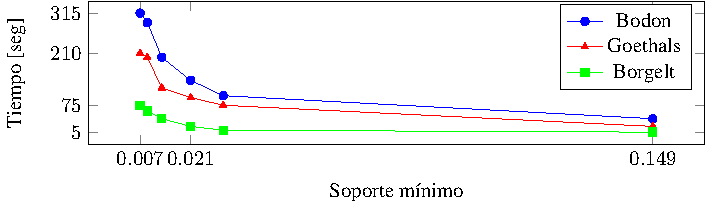
\includegraphics[width=.78\textwidth]{2-1-fig-HCI07-1.pdf}
   \caption{Tiempos de ejecución con la colección \texttt{BMS-POS.dat}}
\label{fig:2-1-apriori-tiemposEjecucionBMSPOS}
\end{figure}

La colección de datos \texttt{BMS-POS.dat} (11.4MB) tiene 515\,597 transacciones con 1\,657 ítems distintos y un total de 3\,360\,020 ítems. Los tiempos de ejecución para valores del \soporte mínimo entre 0.007\% y 0.149\% se muestran en la figura~\ref{fig:2-1-apriori-tiemposEjecucionBMSPOS}.

La figura~\ref{fig:2-1-apriori-tiemposEjecucionBMSView1} muestra los tiempos de ejecución obtenidos al analizar el almacén \D \texttt{BMS-View1.dat} (2.1MB), que contiene 149\,639 líneas con el par $\{$transacción, ítem$\}$ (representación vertical de \D), con 497 ítems distintos. Lo convertimos en un fichero en que cada línea contuviera sólo una transacción (representación horizontal de \D), \texttt{BMS-View2.dat}\footnote{Disponible en el \dvdAdjunto adjunto, en la carpeta \texttt{datos}} (1MB), pues las implementaciones que estamos utilizando leen este formato de ficheros, obteniendo un total de 59\,602 transacciones.

\begin{figure}[htbp]
   \centering
   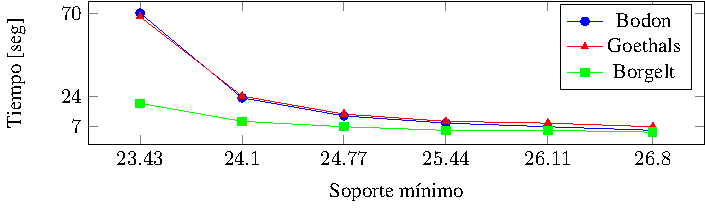
\includegraphics[width=.78\textwidth]{2-1-fig-HCI07-2.pdf}
   \caption{Tiempos de ejecución con la colección \texttt{BMS-View1.dat}}
\label{fig:2-1-apriori-tiemposEjecucionBMSView1}
\end{figure}

Los datos propios (5.1MB) recogían 585\,149 transacciones con 2\,213 ítems distintos y un total de 1\,732\,617 ítems. Los tiempo de ejecución de las implementaciones puestas a prueba con este almacén \D se muestran en la figura~\ref{fig:2-1-apriori-tiemposEjecucionNuestrosDatos}, con \soporte mínimo entre 0.51\% y 17.09\%. En este caso se observan tiempos de ejecución muy grandes (alcanzando los 11 minutos al usar la implementación de Goethals con \soporte mínimo del 0.51\%), lo que pone en evidencia, al compararlo con los tiempos de ejecución de \texttt{BMS-POS.dat}, que además del número de transacciones y de datos a procesar (este último almacén \D contiene el doble de datos que el nuestro) en los procesos de \arm son importantes las relaciones presentes en sus ítems, es decir, puede afectar más al análisis la propia distribución de los datos que su cantidad.

\begin{figure}[htbp]
   \centering
   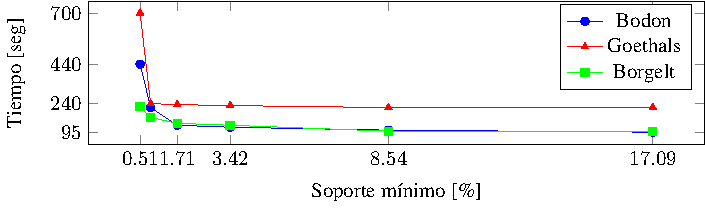
\includegraphics[width=.78\textwidth]{2-1-fig-HCI07-3.pdf}
   \caption{Tiempos de ejecución con la colección de datos propios}
\label{fig:2-1-apriori-tiemposEjecucionNuestrosDatos}
\end{figure}

La implementación de Borgelt, realizada con \langC, era la más eficiente de las tres en todas las ejecuciones excepto para valores intermedios del \soporte mínimo (entre 1.71\% y 17.09\%) en el análisis de nuestros datos en que los tiempos son sensiblemente menores al usar la implementación de Bodon.

Los resultados fueron tan dispares que nos sumergimos en el código usado para analizar el porqué de estas diferencias y poder aprovechar alguna de ellas para introducir nuestras aportaciones o bien crear una nueva implementación con lo mejor que pudiéramos extraer de cada una de ellas. Descubrimos que todos tenían alguna parte mejor implementada que las otras, pero intentar modificarla no parecía fácil a pesar de que Bodon estaba replanteando su trabajo para trabajar con estructuras más modulares, las clases y librerías que aporta el lenguaje \langCpp, ganando en legibilidad a cambio de perder la velocidad de \langC.

Al repasar el código e intentar modificar algunos de sus aspectos descubrimos ciertos procesos que podían optimizarse fácilmente, lo que nos llevó a una nueva publicación, por primera vez en una revista de impacto, descrita en la siguiente sección.